% This is a sample LaTeX input file.  -*- eval: (auto-fill-mode 0); eval: (ispell-minor-mode 1); -*-
%
\documentclass{pasa}%

\title[title]{Economic impact of Demand Response in a wholesale spot market: A case study from the Australian National Electricity Market}
\author[Author1 et al.]{Author1$^1$, Author2$^2$, Author3$^2$ \and Author4$^{2,}$\thanks{This is an example of author footnote}\\
\affil{$^1$This is  an example of Affiliation for Author 1}%
\affil{$^2$This is  an example of Affiliation for Author 2}}%
%%
\jid{PASA}
\doi{10.1017/pas.\the\year.xxx}
\jyear{\the\year}

% UNCOMMENT THE LINES BELOW IF YOU WISH TO USE BIBTEX
%Citations may be made using the natbib commands \citet{},\citep{} etc.
\usepackage[authoryear]{natbib}
\bibliographystyle{unsrtnat}
%\bibliographystyle{pasa-mnras}
\bibpunct{(}{)}{;}{a}{}{,}
\setlength{\bibsep}{0.3mm}

\usepackage[utf8]{inputenc}
\usepackage{fourier}
\usepackage{array}
\usepackage{booktabs}
\usepackage{tabularx}
\usepackage{makecell}
\usepackage{graphicx}
%\newcolumntype{x}{>{\raggedright\arraybackslash}X}
\newcolumntype{Z}{ >{\centering\arraybackslash}X }
\renewcommand\theadfont{\bfseries}
%\renewcommand\theadalign{cc}
\usepackage[autolanguage, np]{numprint}
\usepackage{amsmath}
\DeclareMathOperator*{\argmin}{argmin}
\usepackage{aas_macros}
\usepackage{hyperref} 
\hypersetup{colorlinks,citecolor=blue,linkcolor=blue,urlcolor=blue}
\usepackage{color}
\definecolor{green}{rgb}{0,1,0}
\providecommand{\comment}[1]{\color{green}#1}

\begin{document}%
%
\begin{abstract}
Due to increasing costs of peak power generation and retiring base load power generation, integration of demand response allows for better financial benefits and the management of energy resources in a spot market in the Australian National Electricity Market. Three different levels of DR penetration are analysed in this study in two distinct market conditions based on historic Victorian spot market data in 2014 and 2018 to indicate the most cost-effective DR level and the implications to merit-based spot electricity market. This retrospective analysis manifests that the market could have acquired its accumulated financial savings of A\$120 M - 439 M, which equivalent to relative savings of 5 - 10\% in 2014 and 2018, respectively. The evaluation with the respective data establishes policy implications: the rational size of Demand Response as higher penetration of Demand Response is not always granted greater savings, and prudent time of interventions.

\end{abstract}
%
\begin{keywords}
Demand Response -- Load shifting -- Economic benefit -- Spot market -- Demand Response Policies
\end{keywords}
%
\maketitle%
%
\section{INTRODUCTION}
\label{sec:intro}
\subsection{Background}
In large parts of the world, energy systems are at a critical turning point as the key policy objectives i.e. energy security, affordability, economic development and environmental targets are potentially in conflict with each other. The rising uptake of renewable resources and the onset of digitalisation in the electricity system have made energy transition smoother, however the necessity of integrating demand-side participation and energy storage to harmonising these objectives is often overlooked by the policy makers \cite{crossley2011}.
 
Electricity generation is the largest source of carbon emissions in Australia \cite{finkel2017}, the associated integration of renewable resources has a significant role to play in the NEM i.e. alleviating carbon emissions and lowering levelised cost of electricity. However its intermittent nature poses a reliability challenge to the entire system, as does the decreasing reliability of aged baseload power plants. With higher penetration of renewables, more active grid stabilisation will be inevitable. A favourable option to overcome such problems is provided by the concept of Demand Response.



\subsection{State of knowledge and scope of work}
Demand Response (DR) is widely adopted at the beginning of the 21\textsuperscript{th} century. It is usually used as a mechanism to change the load profile, reduce costs, or improve grid stability. It relies on end-users' participation and responsiveness. It can provide economic benefit for both the consumers and the utility \cite{eu27,vardakas2015,siano2014}.

A considerable amount of literature focuses on applications of DR for specific loads or end-use customers, predominantly behaviour change interventions through pricing incentives for  residential end-use \cite{henley1994,george2002, herter2007,wang2011,torriti2013,downer2016}. Interruptible load or direct load control studies are often limited to a small number of participants \cite{alizadeh2012,vandoorn2015,zaidi2010}. Both approaches employ incentive schemes for customers, encouraging them to reduce their load in response to price signals of various kinds. While the first approach suits residential customers, the latter approach is more practical for industrial users with more stable load patterns \cite{vardakas2015}.

Comprehensive studies of DR application to optimise both energy consumption and price are often restricted to a limited number of participants \cite{mohsenian-Rad2010,pipattanasomporn2012,valogianni2016}. Few studies have addressed the merits of DR concerning reliability improvement and environmental mitigation \cite{wang2017}. While the application of DR has been a focus in smart grid or energy future research, less research has been conducted about the changes caused by load shifting, load shedding at state / national level \cite{markle2018}. Moreover, a subtle yet intriguing element of DR application in relation to flexibility of demand and price volatility in electricity trading markets has been neglected in mainstream research because DR is traditionally regarded as incentive measures to reduce demand.

In this research we investigate the potential impacts from DR deployment at state level, based on real bid/offer data in the spot trading market within the Australian National Electricity Market in 2014 and 2018. In addition to estimating costs potentially recovered by reduced use  of peak gas-fired generation, we compare seasonal variation of the wholesale prices between summer and winter. To reflect the increasing uptake of demand response in the future, we simulate scenarios that reflect varying rates of increase in penetration of DR as a percentage of historical maximum demand trends.

\section{THE SPOT MARKET IN THE AUSTRALIAN NATIONAL ELECTRICITY MARKET}
\label{sec:NEM}

The Australian National Electricity Market (NEM) is an energy-only market where prices are set under a uniform price auction, with a merit order based market clearing mechanism. It comprises five state-based New South Wales (NSW), Victoria (VIC), Queensland (QLD), South Australia (SA) and Tasmania (TAS), with inter-connectors between. Across the NEM, around 80\% of the generation fleet is privately owned with a few publicly owned generators mainly located in Queensland, while transmission and distribution networks are predominantly owned by state governments and retail providers are privately owned \cite{aer2019}. The Australian Energy Market Operator (AEMO) operates the connection of electricity between generators and consumers. 

\begin{figure}
\begin{center}
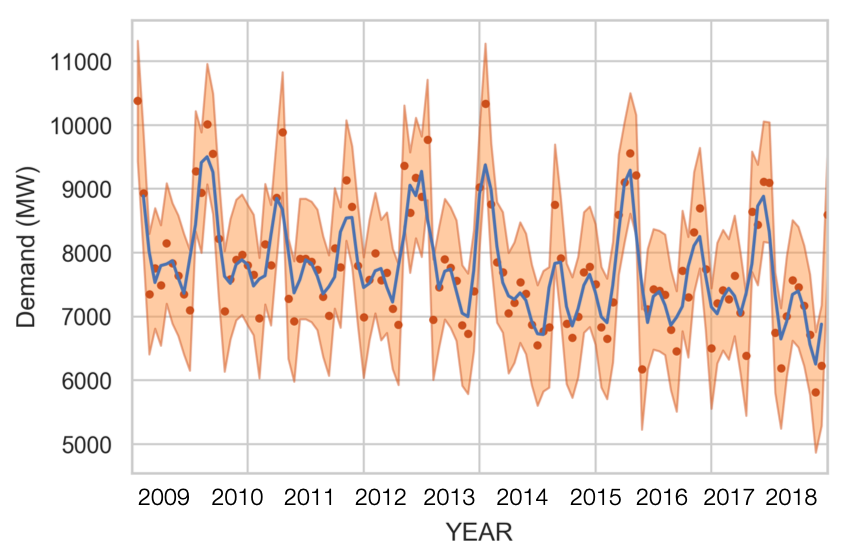
\includegraphics[width=.7\textwidth,height=.23\textheight,keepaspectratio]{DR/PASA_example/Figures_DR/vicmaxdemand.png}
\caption{Monthly maximum demand in Victoria between 2009 and 2018}\label{fig:Fig1-vicmaxdemand}
\end{center}
\end{figure}

Within Victoria, the record peak demand is 10,490 MW, with an average annual demand of around 5,100 MW (summer 2014 to summer 2019). Peak demand usually occurs in either January or February, exceeding winter peaks by 1.5 GW (see Table~\ref{tab:table1}). Summer peaks have a slight downward trend from approximately 9,950 MW during (2008-2013) to around 9,070 MW (during 2014-2019) due to a remarkable rate of solar rooftop uptake (See Figure~\ref{fig:Fig1-vicmaxdemand}). However, the possible maximum demand at the 1-in-10 years probability of exceedance in 2021-22 (or POE 10\%) is expected at 9,859 MW \cite{aemo2018}, with a tight installed capacity of 10,383 MW including 1,100 MW intermittent resources (Jan 2019).

Unlike commodity markets, electricity prices are highly volatile and abruptly changed due to the effect of \textit{mean-reverting} \cite{escribano2011}. If demand increases, generators with greater marginal costs will enter the market with significantly higher price offers, pushing higher wholesale prices. When demand returns to average levels, these generators will be pushed off the bidding table and prices will fall \cite{ignatieva2016}. Likewise, price spikes are also induced by extreme weather events. Within the events, electricity demand typically surges in a short period of time, all available generators, including inter-connectors are recruited to  meet demand and  wholesale prices are generally bid close to the market price cap (\$14,2000 per MWh). 
\cite{Higgs2009} indicated that the Australian spot market is more prone to price spikes than other electricity markets, and hence it creates a higher divergence between the spot prices and demand during demand surge periods. In comparison to other energy-only markets e.g. Electric Reliability Council of Texas (ERCOT) and Energy Market Authority of Singapore (EMA), the spot market in Australia has a considerable sharp spike during the peak load period (See Figure~\ref{fig:Fig2-allloadcurve}). The spot market in singapore shows a high utilisation rate, where the trough to peak ratio is low and the loads are distributed fairly evenly; whereas the spot market in Texas features a relatively flat base load period with a steep intermediate load.

In addition to the mean reversion effect, the spot market also exhibits seasonal variations with higher price spikes during summer despite lower weighted average prices throughout the season. This can be interpreted that the electricity market in Australia has a non-linear supply-demand nature.

\begin{figure}
\begin{center}
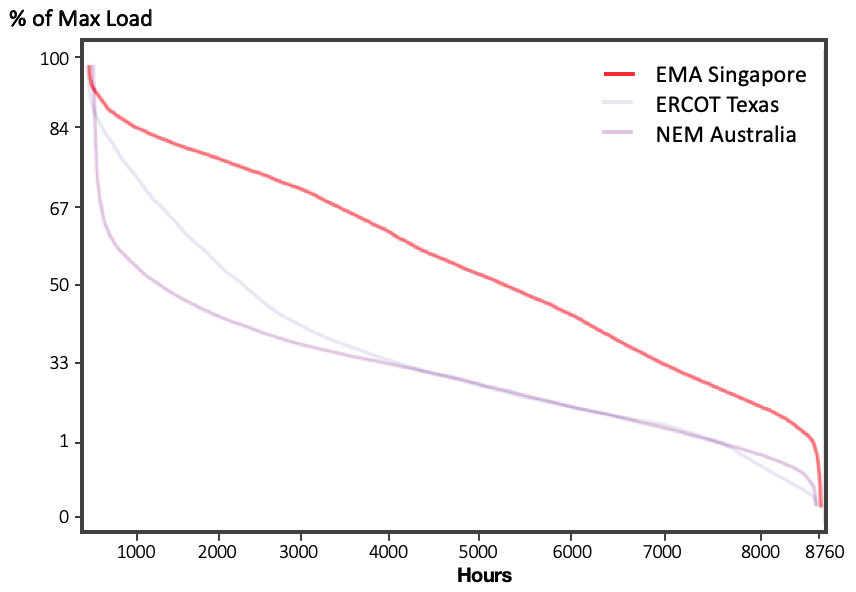
\includegraphics[width=.7\textwidth,height=.23\textheight,keepaspectratio]{DR/PASA_example/Figures_DR/allload.png}
\caption{Comparison of load duration curve in 3 energy-only markets in 2018}\label{fig:Fig2-allloadcurve}
\end{center}
\end{figure}

\begin{table}[]
\caption{Maximum and average demand profiles in Victoria between 2013 and 2018.}
\begin{center}
\label{tab:table1}
\begin{tabular}{p{0.7cm} ccc}
\cline{1-4}
 & \multicolumn{3}{c}{\textbf{Electricity Demand in Victoria}} \\ \cline{1-4}
 & \begin{tabular}[c]{@{}c@{}}Winter peak \\ demand\\ (MW)\end{tabular} & \begin{tabular}[c]{@{}c@{}}Summer peak \\ demand\\  (MW)\end{tabular} & \begin{tabular}[c]{@{}c@{}}Average annual \\ demand \\ (MW)\end{tabular} \\ \cline{1-4}
2013 & 7,898 & 9,760 & 5,272 \\
2014 & 7,648 & 10,308 & 5,321 \\
2015 & 7,923 & 8,635 & 5,193 \\
2016 & 7,767 & 9,523 & 5,079 \\
2017 & 7,472 & 8,730 & 4,953 \\  
2018 & 7,874 & 9,159 & 4,948 \\ \cline{1-4}
\end{tabular}
\end{center}
\end{table}

In ordinary operation of the Australian spot market, the market is established through a 'pool' which  aggregates the output from all generators and matches forecast five-minute demand. The market dispatch algorithm selects from the lowest price offer to the highest, and then bids are stacked until capacity is met. To account for forecast error or unprecedented events, excess capacity from the pool is contracted within minutes to meet the demand. Although the bid is finalised every five minutes, the 30-min average is  used as the final wholesale price. Often in periods when demand is reduced, electricity prices fall. Due to the operating cost or constraints of generators, that cannot adjust to the new demand level, also negative price spikes can occur \cite{fanone2013}. This open up opportunity for large industry users to participate by curtailing their loads for short periods in response to demand spikes \cite{aemc2017}.

The generation fleet in Victoria still relies heavily on fossil-fuel plants, which account for 7,040 MW or approximately 70\% of the total installed capacity, despite the decommissioning of the 1,600~MW coal-fired, Hazelwood station. Of these, around 2,400 MW is gas-fired, while hydro and renewables account for around 2,200 MW, and 1,100 MW, respectively. In 2018, there were 337 occurrences when the pool prices were at double or more than the annual average wholesale price. Of the total occurences, there were 133 times that forecast demand fell short of the actual demand. It is noteworthy that the wholesale prices in Victoria have risen around 60 - 80\% after the closure of the 1,600 MW Hazelwood power station in early 2017 \footnote{Hazelwood power plant used to account for 18\% of the total installed capacity in Victoria}, albeit it was largely superseded by newer power sources.

\section{FINANCIAL BENEFITS FROM DEMAND RESPONSE}
\label{sec:financial}
Preliminary studies generally conclude that demand response has  many positive effects. These include economic and environmental benefits, as well as improvements in pricing, risk management, reliability and market efficiency

The deployment of Demand Response has proven to be a cost effective and reliable approach to deal with uncertainty in system reliability. The benefit of DR is even more pronounced when allied to the deployment of advanced metering infrastructures. Some preliminary work such as (\cite{faruqui2010,ofgem2010}) quantified the economic impacts of combining smart metering with DR. However these studies rely heavily on assumptions in participation rates. While a large body of literature \cite{faruqui2012,lawson1992,filippini2011,henley1994} examine the s of time-of-use pricing mechanism, empirical study from Northern Italy was in contradiction with the findings suggested in the above experiment, as it underlined that the introduction of time-of-use tariffs failed entirely to alleviate and shift the peak demand \cite{torriti2012}. It was not until recently that \cite{muratori2016} proposed the solutions to resolve the rebound peak effect of static time-of-use pricing scheme. The methodology involved multi-stage pricing, coupled with large-scale adoption of automated scheduling frameworks on the aggregate demand with electric vehicles. This model was able to cope with the rebound peaks created by the synchronisation of the individual residential demands and resulted in 12\% to 17\% of demand reduction.

A key problem with much of the literature on a larger scale price-based DR is the uncertainties in adoption of the energy intensive appliances i.e. heat-pumps or electric vehicles. An Austrian case-study \citep{prggler2012}  involved a wide range of household appliances, heat pump and electric vehicle charging. This study highlighted a potential saving between 1 euro and 6 euro per year can be attained from a  general household in Austria. However, load shifting of 15\% is granted in this study.

In Europe, DR has been progressively expanded and adopted through retailers with limitation for aggregators even in most advanced member states \cite{bertoldi2016}.  \cite{feuerriegel2016}  reported that  savings of 3.11 million euro or 2.38\% can be achieved from load shifting  in the residential and  service sector in Germany. A more comprehensive study in Germany \citep{hcgils2016} found that DR can potentially reduce the unit cost of electricity from 38.1 Euro/MWh to between 36.8  and 37.6 euro/MWh  equivalent to an annual saving of around 377 million euro. Information collated predominantly from several UK governmental institutions reported that a reduction of demand of 4\% can be achieved from DR which can be translated to 286 million GBP of annual savings \cite{bradley2013}. Even though research has focused on the economic aspects of DR, only a limited number of studies have considered the real spot market data. \cite{markle2018} studied DR in the German and Austrian spot markets. They noted potential cost savings of up to 500 million euro or 6\% of the market expenditure in 2014. This study not only assumed the level of flexible loads of 25\%, but also assumed a linear relationship between price and demand.

In summary, the financial benefit of DR in real-world spot markets has been little investigated. Previous DR integration works have largely focused on either incentive measures or automated DR technologies. However they failed to address both (1) the pragmatic level of DR penetration in specific spot market, and (2) the correlation of the load shifting / shedding associated with its economic benefits. Therefore, quantifying economic benefits of DR in a spot market are investigated further in this research.



\section{MODEL DESCRIPTION AND FORMULATION}

This section presents our model formulation for investigating the impact of statewide DR potential. The study was conducted in three steps. First, load duration curve and distribution of cumulative price as percentage of hours are identified \hyperref[sec:model4.1]{(Section 4.1)}. In the second part, their characteristic load profiles are assessed \hyperref[sec:model4.2]{(Section 4.2)}. 
Finally, optimisation of load shifting and balancing is investigated, and the potential cost savings after the market clearing are quantified \hyperref[sec:model4.3]{(Section 4.3)}. 

\subsection{Identification of electricity loads and prices in Victoria}
\label{sec:model4.1}

As the National Electricity Market in Australia is  an energy-only market, generators are only paid for their energy dispatched, not  their available capacity. To cope with uncertainties and variations in the generation and demand, the installed capacity must be  larger than the historical maximum demand or 1-in-10 years weather events.
 
Historically, baseload electricity was dispatched by the most reliable and inexpensive power plants i.e. Brown coal. The market  now employs a merit order dispatch system so that   dispatched energy is stacked based on ascending order of price. Thus intermittent power from wind and solar  sometimes replaces some incumbent power sources \cite{aer2010}. 

When neglecting ramping constraints, the bottom of the electricity load curve in Victoria is composed of generators that have lowest marginal costs such as brown coal or renewable resources. Intermediate load is often supplied by fuels such as brown coal (excess from baseload), hydro, gas and some power brought from interstate. The most expensive peak load is usually fed by open cycle gas turbine or combined cycle gas turbine plants.
\begin{figure}
\begin{center}
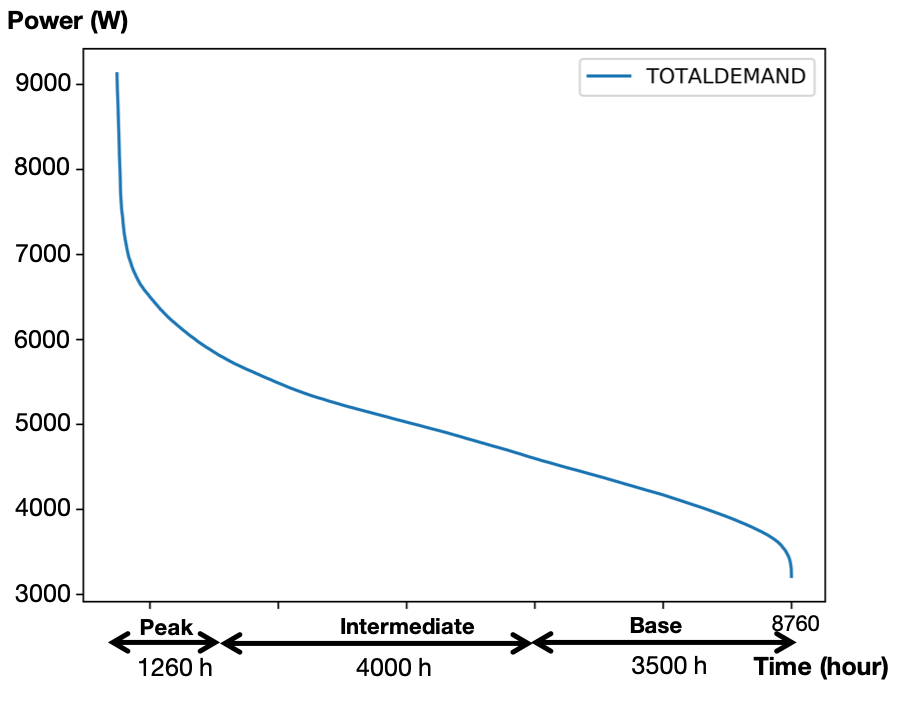
\includegraphics[width=.7\textwidth,height=.28\textheight,keepaspectratio]{DR/PASA_example/Figures_DR/loaddurationcurve_2018.png}
\caption{Load duration curve in Victoria 2018}\label{fig:Fig3-loadcurve}
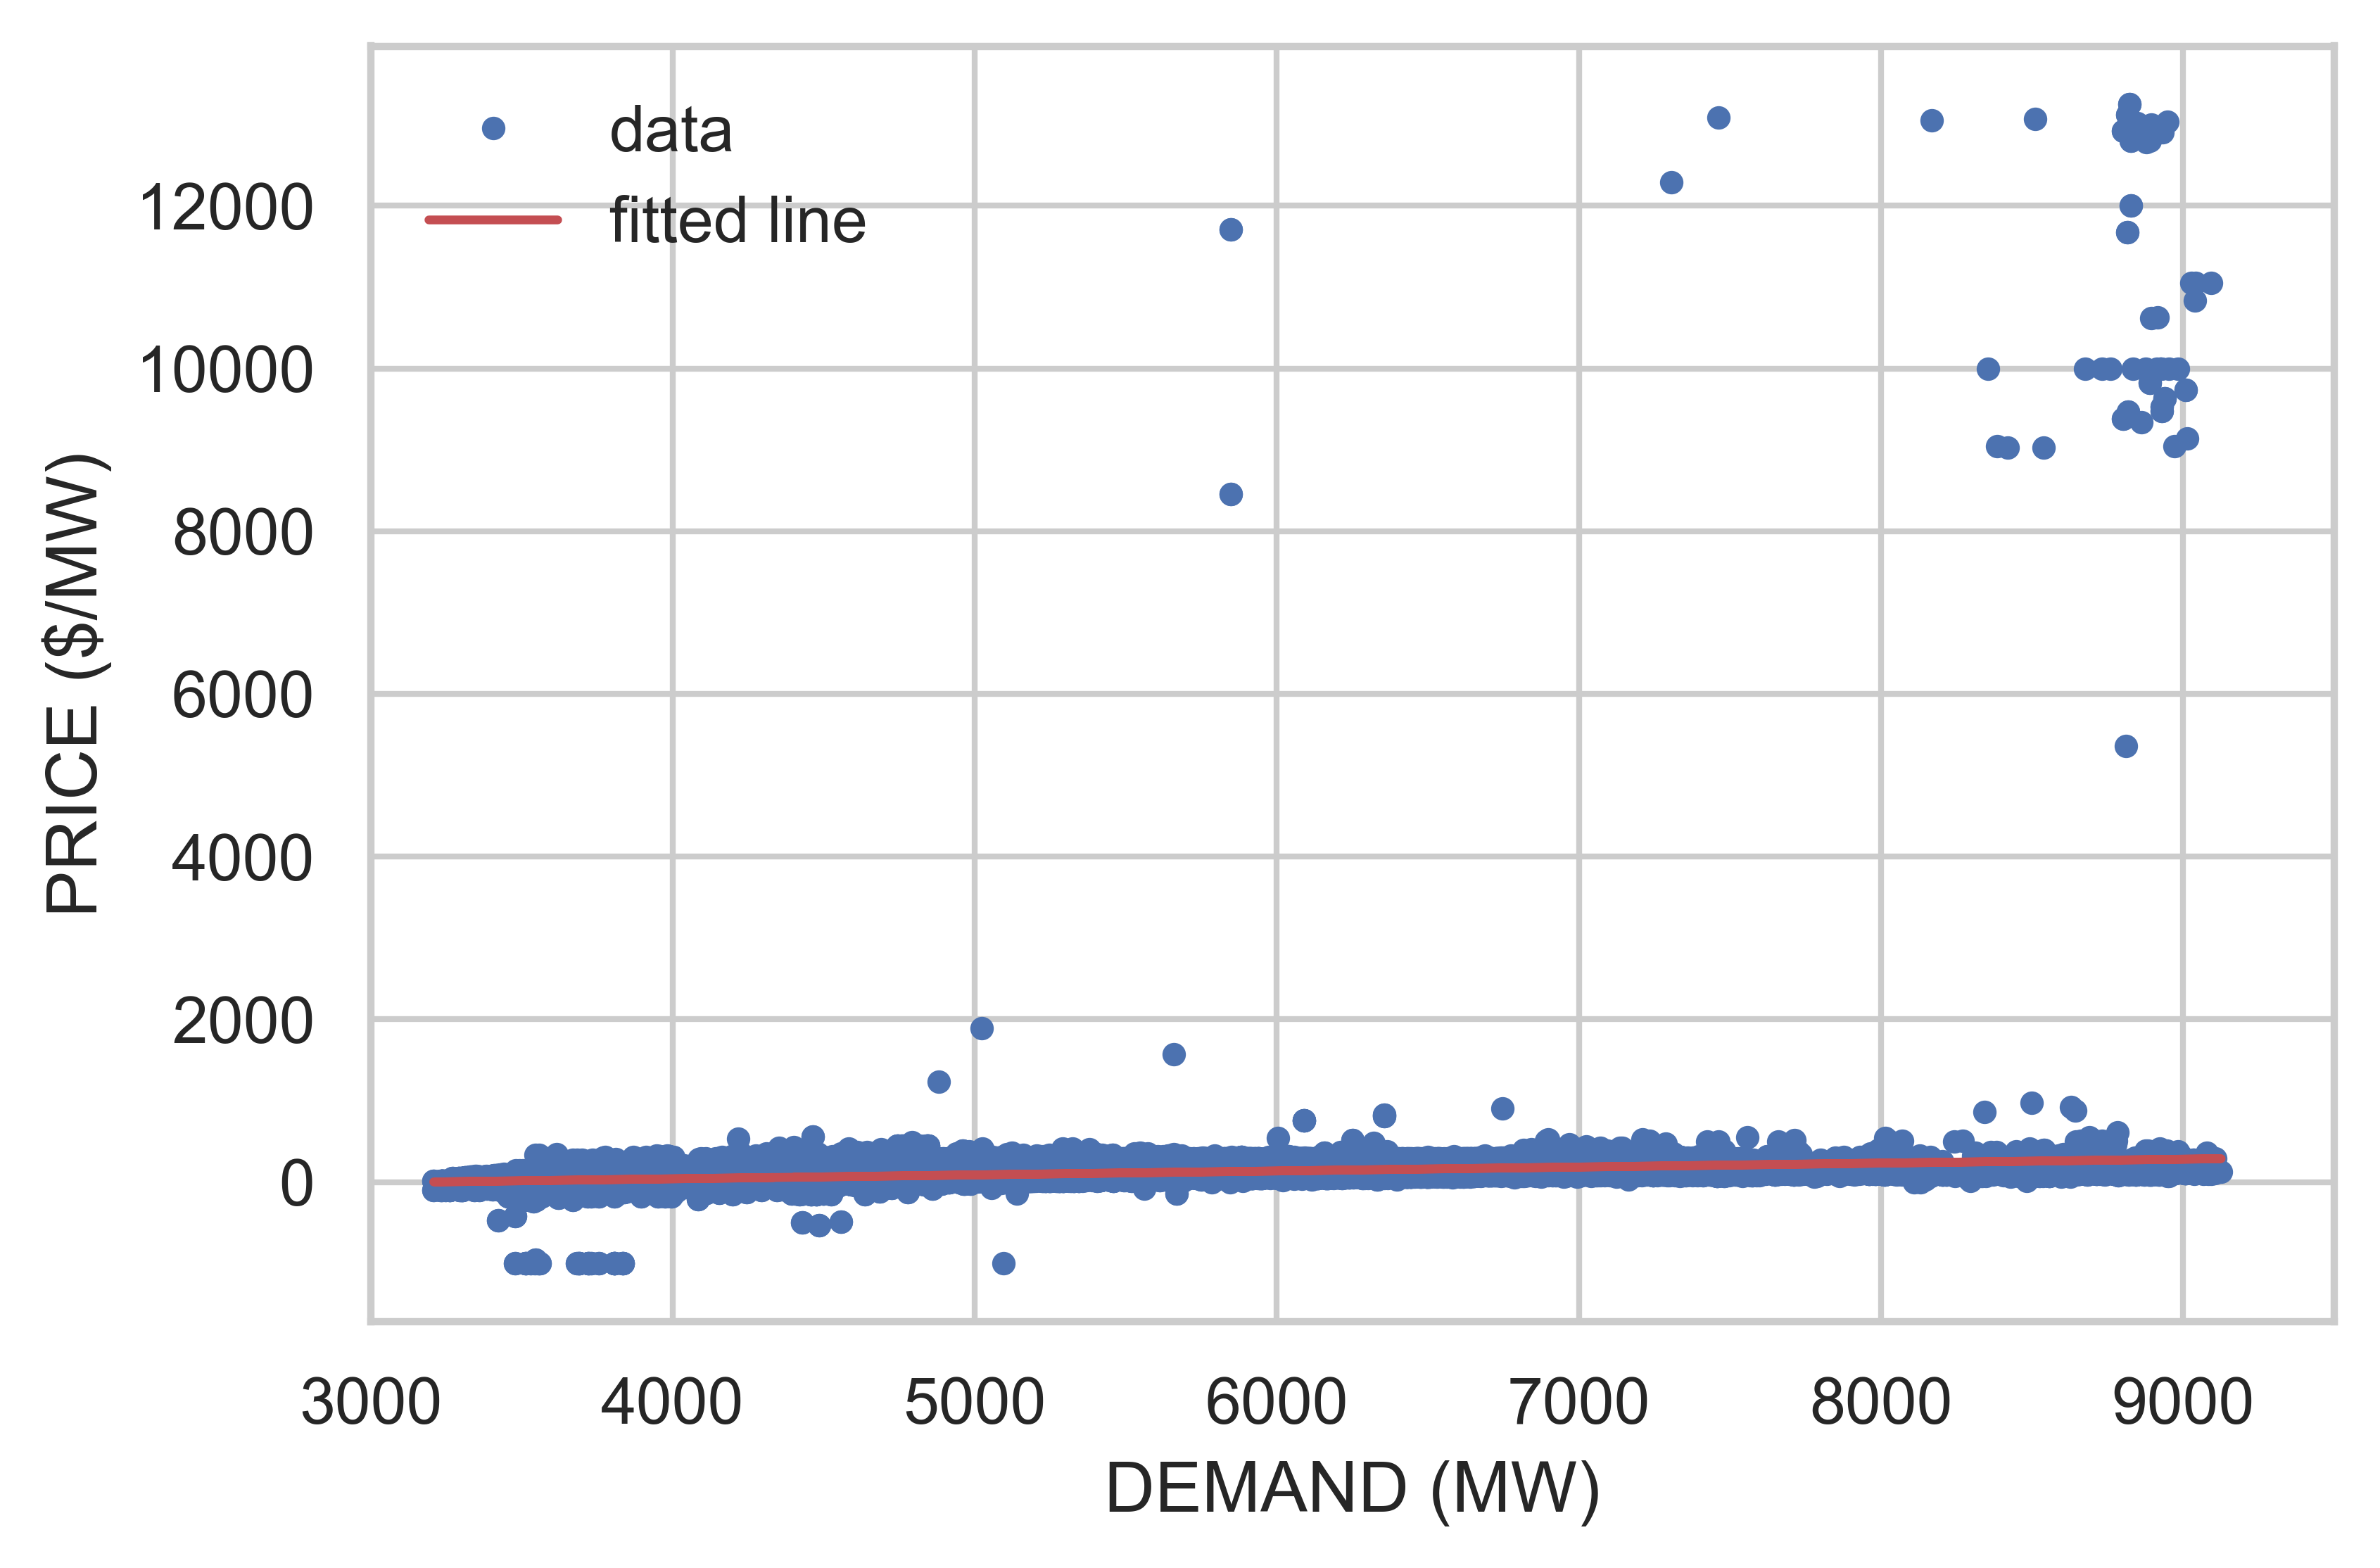
\includegraphics[width=.7\textwidth,height=.23\textheight,keepaspectratio]{DR/PASA_example/Figures_DR/price2018.png}
\caption{Price and demand relationship in spot price market, Victoria 2018}\label{fig:Fig4-pricedemand}
\end{center}
\end{figure}

Highly flexible power plants are generally required only when the loads surpass 5,000 MW or when renewable and hydro power are not available.  These technologies have high  operational and maintenance costs \cite{aer2018}. The relationship of the demand curve and prices is presented in Figure~\ref{fig:Fig3-loadcurve} and Figure~\ref{fig:Fig4-shiftingwindow}. It is evident that the demand and price relationship becomes exponentially inelastic when demand is higher. In higher demand events, a merit based selection is less effective as generators with higher variable costs and shorter ramp-up time such as older natural gas steam turbine generators are recruited. In addition to price spikes in higher demand events, most prices can be expected as low as the annual volume weighted average price due to sufficient supply and market hedging in 30-min settlements market (described in details in \hyperref[sec:NEM]{(Section 2 - the NEM)}.

\subsection{Demand-supply and price model from the spot market}
\label{sec:model4.2}

The Australian Energy Market Operator (AEMO) uses a number of constraint equations to develop the national market dispatch algorithm. In consonance with  AEMO's dispatch algorithm, the price for each region is determined every 5 min, and the 6 dispatch prices in a half-hour period are averaged to determine the regional spot price for that half-hour trading interval. This model obtained pristine data-set from a publicly available AEMO's database. Five-minute settlement data of dispatched electricity and price was employed, representing 104,382 trading intervals in 2018 (there are 288 missing data on that year). The data was then fed to the model and is recalculated on a 30 minute basis, per specified rules.

In essence of the normal operating state in the NEM, constraints such as minimum ramping up / down rates are crucial for the market operation. Factors concerning operations of long ramp-up rate plants such as thermal plants (coal) would under most circumstances be expected from the algorithm. Other important constraints emerge when generators are bound to establish efficient supply of electricity, including constraining generation off or on. Under `constrained off' condition, a generator is bound to decrease its output at a level below what would otherwise be expected from the dispatch curve based on marginal costs, and it may be unable to obtain a potentially higher market return by increasing its energy production. In order to balance supply, higher merit ranked generators (would not be dispatched in normal operation) are forced to provide energy at a higher merit level, usually at a level that is more costly than the market return. This condition is defined as `constrained on', which has a negligible impact to the market clearing prices \cite{aemoconstraint2013}.

The dispatch algorithm incorporates long-term and short-term forecast of demand, generation capabilities in different regions; generation and interconnection constraints; meteorological data; as well as frequency control ancillary services. These constraints put together to ensure the security provision of the electricity system, the maximum value of trade subject to different limitations in the main dispatch process \cite{aemo2019}. Even though all the constraints that need to be considered in a specified dispatch interval may not be satisfied within this study, the model outcomes are considered meaningful as costs of these constraints have a marginal impact to the wholesale price, this study otherwise simplifies some constraints undertaken in the NEM.

Given that the NEM spot market generally trades between regions, some marginal losses occur in transmission. This model however omits such costs as well as interconnector costs and considers predominantly the price compensation regaining from DR implementation in the historical bid stack. Albeit the load intervention, dispatch process proceeds from the cheapest electricity (at a given Regional Reference Price, RRP), regularly from plants with lowest marginal costs (e.g. coal, wind and solar) is preferentially dispatched. This assumption essentially bring down the electricity prices, compare to the actual volume weighted average price \cite{aemoloss2019}. 


A growing body of literature has pointed out the positive aspects of DR on pricing, however few studies have literally integrated DR into the spot market. As the Australian spot market is a highly \textit{mean-reverting} market --- generators with greater marginal costs will enter the market with higher price offer, abrupt reduction of electricity demand owing to load shifting or shedding could technically induce the significant decrease of the spot prices. In this model, we assume that retailers or DR providers are fully integrated into the market and are  able to trade in future spot auctions.  

\subsection{Load shifting model to optimise electricity procurement}
\label{sec:model4.3}

In this section, modelling details and parameters are introduced. It comprises all equations and assumptions used in this study. 

\subsubsection{Existing spot market model}

The electricity market expenditures have a high correlation and dependence with electricity demand, temperature and unplanned generation downtime. For the sake of simplification, this model takes into account the strongest factor that induces monetary expenditures i.e. electricity demand. Historical bid stack was utilised to extract raw bid / offer data from generators that supplied energy to Victoria. In this model, electricity demand $D$ is met by supplier $i$ at any time $t$. Each supplier offers power $P$ at specific cost $C$.

Let $D (t)$ denotes the historical demand at time t. At all time, the power output from generators ($P^s_i (t)$) combined has to at least be satisfied with the demand. Given that the power is stacked up based on its price ($C_i (t)$), the relationship of demand based on its merit can be explained in Equation \ref{eq_meritorder}


\begin{equation}\label{eq_meritorder}
D_{i} (t) = \min\limits_{i \in [1,...,N]} \sum_{i=1}^{N} \big( C_{i} \times P^s_i \big),
\end{equation}

In the NEM dispatch market, Supplier $i$ will offer an amount of power $P^s_i$ at price $C_i$. AEMO's algorithm then establishes the bid-stack from lowest to highest price.
AEMO buys an amount $P_i$ of power from supplier $i$. In ideal case, the procurement of $P_i (t)$ should be equal to $D_i (t)$, but the algorithm may not be fulfilled due to size of power offer$P^s_i$. The number of successful suppliers denotes as $M$ is calculated by Equation ~\ref{eq:bidstacksize}

\begin{equation}
  \label{eq:bidstacksize}
  M = \min_K \mathrm{such\ that} \sum_{i=1}^K P_i > D
\end{equation}


AEMO uses the following simplified algorithm to determine settlement --- the harmonising of payments by the electricity consumers and the energy purchased by AEMO from power generators. In equation \ref{eq:expenditure}, let $E (t)$ denotes the market expenditure at time $t$. The algorithm is run every five minutes but actual payments are based on 30-minute averages of regional reference price (RRP). This equation concedes prices within a region to be the same without marginal loss factors.

Thus, the total market expenditure of the spot market is achieved by the summation of regional reference prices $C_{RRP} (t)$ (\$/MWh) from successful offers in the pool auctions and amount of power associated to the costs $P_i (t)$. The reference price $C_{RRP}$ is then set to be $C_M$ and \emph{all} suppliers are paid at this price so that the expenditure is given by

\begin{equation}
  \label{eq:expenditure}
  E (t) = C_{RRP} \sum_{i=1}^M P_{i}
\end{equation}

Where:
\begin{itemize}
    \item [$C_i$] and [$P_i$] are at the discretion of the generators.
    \item [$P_i$] is subjected to a power balance constraint (Power based on  merit of price, subject to \\
    $P_i,min \leq P_i \leq P_i,max,   i = 1,...,N$
\end{itemize}


These algorithms are subject to technical constraints which are not in the scope of this study. We note only that most of the constraints are active when meeting spikes in demand. Our study will generally reduce these spikes so the impact of constraints should be reduced.



\subsubsection{Spot market where demand response (DR) is fully integrated}

The historical data was manipulated to a set of adjusted price based on merit order on a five minute basis, at \(N\) = 288 time slots per day. The load shifting criteria pitch in when the actual demand goes beyond a safe supply threshold \footnote{Derived from the maximum capacity factors of intermittent plants combined with the total installed capacity of baseload plants} (8,500 MW) or the Regional Reference Price (RRP) of \$200 per MWh. Given that the 30 minute settlement is used to determine the market expenditures, maximum price C\textsubscript{max}\((t)\) at each 5 minute time interval is combined and averaged for every 30 time intervals (00:05 - 00:30) is then used to determine the market expenditures. 

From a diagram in Figure~\ref{fig:Fig4-shiftingwindow}, we can see that the duration of load shifting can be moved freely within available time window of $\Delta \textsubscript{j} (t)$ (hr). The equations present in the following sub-section provide the scopes of the load shifting assumptions used in this study. The shifting threshold refer to as $\theta_{max}$ ranges between 250 and 950 MW based on scenario selected. The total load shift away is the summation of the number of shifting occurrence at any time \textit{t}, the shifted load is defined as $\theta_k (t)$, where $\theta_k (t) \leq \theta_{max}$. Let us denote the demand reduction by $D'_{red,k} (t)$. As given by Equations \ref{eq_demandred1} and \ref{eq_demandred2} the demand reduction is defined relative to the potential load shifting presented in Equation \ref{eq_shiftedload}

\begin{equation}\label{eq_shiftedload}
shifted \, load\quad \theta^* (t) = \sum_{k=1}^{T} \big( \theta_k (t) + ... + \theta_n (t) \big),
\end{equation}

Thus, the demand reduction equation can be identified as:
\begin{equation}\label{eq_demandred1}
\sum_{k=1}^{T} D'_{red,k} (t) = \sum_{k=1}^{T} (D_k (t) - \theta_k (t)),
\end{equation}
subject to 
\begin{equation}\label{eq_demandred2}
\theta_k (t) \geq 0 \quad and \quad \theta_k (t) \leq \theta_{max} \qquad for \; t = 1,...,T,
\end{equation}

\begin{figure*}
\begin{center}
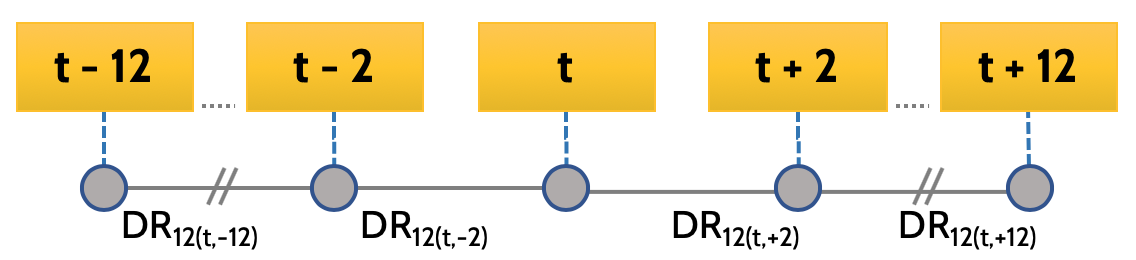
\includegraphics[width=.8\textwidth,height=.5\textheight,keepaspectratio]{DR/PASA_example/Figures_DR/DRtimes1.png}
\caption{Load balancing windows at time t}\label{fig:Fig-shiftingwindow}
\end{center}
\end{figure*}


In order to simulate the impacts of DR in the spot market, load shifting algorithm was introduced in three different scenarios and analysed based on level of DR adoption: 1) High DR is assumed based on a nationwide DR potential study in Germany, around 10\% of maximum demand (950 MW) in Victoria is granted to be shiftable \cite{klobasa2009}; 2) Moderate DR assumes that large commercial and industrial users are readily participated in DR programs, around 6\% of maximum demand is assumed to be shiftable; and 3) Low DR is granted as a business as usual scenario where no active DR entities are eagerly participated in the market, thus around 2.5\% of maximum load is projected to be shiftable.

\subsubsection{Load balancing model with market clearing mechanism}\label{loadbalancing}

As the load is assumed to be 100\% utilisable for any load under that falls under our specified criteria, this allows the model to shift the loads forward or backward within 24-hour time window as displayed in Figure~\ref{fig:Fig4-shiftingwindow}. The load shifting equation used bear a close resemblance to the one proposed by \cite{feuerriegel2014}. However, the algorithm used in this study is established to filling up the trough within a specified time-window. The load shifting problem can be posed on terms of maximum time prolonging or advancing denoted by \textit{j}. As this model is granted loads to be balanced within 24 hours, i.e. j\textsubscript{max} = 12h. Let DR\textsubscript{j}(t, t\textquotesingle - t) identify the shifted load between hours t and t\textquotesingle. If t\textquotesingle is less than t, then the load is shifted to the advanced point in time where the electricity demand is lower and vice-versa when t\textquotesingle is greater than t. For example, DR\textsubscript{12}(t,-3) stands for load that has an advanced shift of 3 hours within the maximum shifting time between -12 and + 12 hours. From the diagram in Figure~\ref{fig:Fig4-shiftingwindow}, it can also be interpreted that at time \textit{t} loads are reduced by DR\textsubscript{1}(t,0) till DR\textsubscript{12}(t,0) with the maximum reduction of $\theta_{max}$.


In order to ensure that the total demand remains virtually unchanged by the shifting mechanism throughout time \textit{t}, the original electricity demand $D_i (t)$ is manoeuvred by $D'_{red,k}$ (demand reduction) and re-balanced with $D'_{inc,i}$ (demand increase) which have identical summation. The total potential demand increase according to demand reduction in DR\textsubscript{j}(t,0) is increased by the sum of $DR_j (t+i, t'-t)$. Considering that the shifting threshold $\theta_{max} (t)$ can be huge and unlikely to be discharged all at once, the model splits each shifted load into 6 identical parts and continually fills up the points in time where demand is lowest which can be derived by the following constraint:

\begin{equation}\label{eq_loadbalancing1}
\sum_{i=1}^{M} DR_{bal,j} (t) = \frac{1}{6} \sum_{i=1}^{M} \big( \theta_i (t) + ... + \theta_m (t) \big),
\end{equation}

where the balancing DR term is derived by Equation \ref{eq_loadbalancing2}:
\begin{equation}\label{eq_loadbalancing2}
\theta^* (t) = \sum_{t - M}^{t + M} DR_{bal,i} (t)
\end{equation}

The balancing equation then iterates by the following steps until each in $\sum_{i=1}^{M} DR_{bal,j} (t)$ is depleted:
\begin{enumerate}
\item The algorithm seeks for the minimum demand within $DR_{12} \, (t, t'- t)$ or 12-hour window of the load to be shifted $\theta^* (t)$ and fills with a fraction of $DR_{bal,j} (t)$ based on Equation \ref{eq_loadbalancing1}.
\item The algorithm iterates and distributes the amount left in $\theta^* (t)$.
\item The algorithm iterates the above procedures until the demand shifted away is depleted.
\end{enumerate}

This term is only limited to the shiftable load, or a shift from t to t\textquotesingle by $DR_j (t, t'-t)$, to this extent $DR_j (t, i) = 0$ where t + i < 1 or t + i > 12. 

Collectively, the modified demand at any time $D'_i (t)$ is given by:

\begin{equation}\label{eq10}
D'_i (t) = D'_{red,i} (t) + D'_{inc,i} (t)
\end{equation}

With regard to the realistic estimates of the potential savings, the historical demand and price profiles in 2014 and 2018 were analysed. In order to calculate the wholesale spot prices that incorporated the impact of DR using the model described above, a set of modified prices was generated based on a set of modified demand profiles. The model however was not considered the original offers from the pool, instead it relied on the historical prices from the 5 minute settlement. The 5-min settlement prices associated with the shifted demand were then superseded with the modelled prices and averaged over the half hour trading interval to yield the new spot price for every 30-min time interval. As the model simply shift a small block of power at a time, the additional costs based on shifted demand is marginal. At lower demand, the relationship between price and demand shows a strong correlation of linearity. The model employs least squares approach to produce the modified prices at each shifted time block.

Hence, accumulated potential savings gained from DR can be induced from the differences between the actual market expenditures $E_{EXT} (t)$ and the total market expenditures $E_{DR} (t)$ under different DR scenarios.

\begin{figure*}
\begin{center}
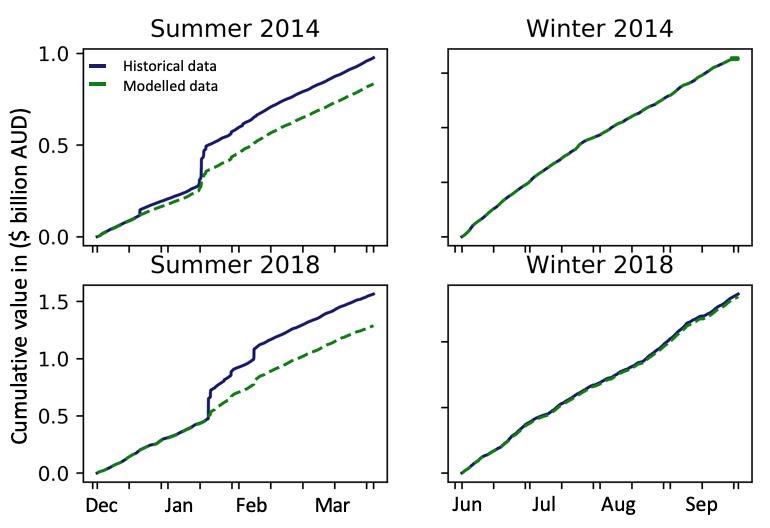
\includegraphics[width=.9\textwidth,height=.5\textheight,keepaspectratio]{DR/PASA_example/Figures_DR/Cumsea01.png}
\caption{Comparison of market expenditures with load shifting and the effect of seasonal variations in 2014 and 2018}\label{fig:Figseasonal}
\end{center}
\end{figure*}

\section{RESULTS AND DISCUSSION}

In the following section, we provide the evidence that the penetration of Demand Response can bring down the overall wholesale costs. Furthermore, we simulate the financial benefits of Demand Response and relate our results to existing literature and ultimately compare these across each scenario.


\subsection{The price characteristics and demand response potential}
\label{sec:dis5.1}

In order to obtain the most realistic model configuration, the model employed the pristine demand and price profiles predominantly used by Victorian electricity users. This allows for valid and credible rationale to be derived from the study. This dataset entails approximately 2.7 million households with the aggregated consumption of around 46 TWh or 23\% of the total annual electricity consumption in the NEM. \footnote{The total electricity consumption in Australia was around 202.5 TWh in 2018 source:\cite{opennem2019}} Although not all constraints applied by the market operator is fulfilled by this model, the model outcomes are worthwhile for the wholesale demand response study.
The model output was validated and compared with real data in the two respective years (2014 and 2018). These two years were chosen to examine the market impacts associated with decommissioning of baseload power plant. The cumulative traded value is used to stress the patterns of price spikes during normal and important weather event periods as this approach has a unique ability to unveil the ambiguity of the price and demand relationship. 

Even though all the constraints that need to be considered in a specified dispatch interval may not be satisfied within this study, the model outcomes are considered meaningful as costs of these constraints have a marginal impact to the wholesale price, this study otherwise simplifies some constraints undertaken in the NEM.

The model presents in this section is based on the moderate DR scenario (scenario B). From the historical price events, even though the price surges are blatantly stand out from the load curves, adopting price accumulation is ideal for tracking the long-term variation of price indicators. From Figure~\ref{fig:Figseasonal}, it is noticeable that the fluctuation in spot price is higher in summer and lower in winter. While the cumulative prices increase gradually in winter, sharp increases of price occur in summer and hence the magnitude of potential savings is higher in this season. It is noteworthy that the retirement of the 1.6 GW coal-fired power plant leads to the increase in the total expenditure of about 50\% between 2014 and 2018. By applying DR, it would induce savings of \$273M (14\%), \$529M (16\%) in summer 2014 and 2018, respectively. Anyhow, a mere 0.2 - 1.4\% of the total market savings can be achieved in winter of both years.

\begin{figure}
\begin{center}
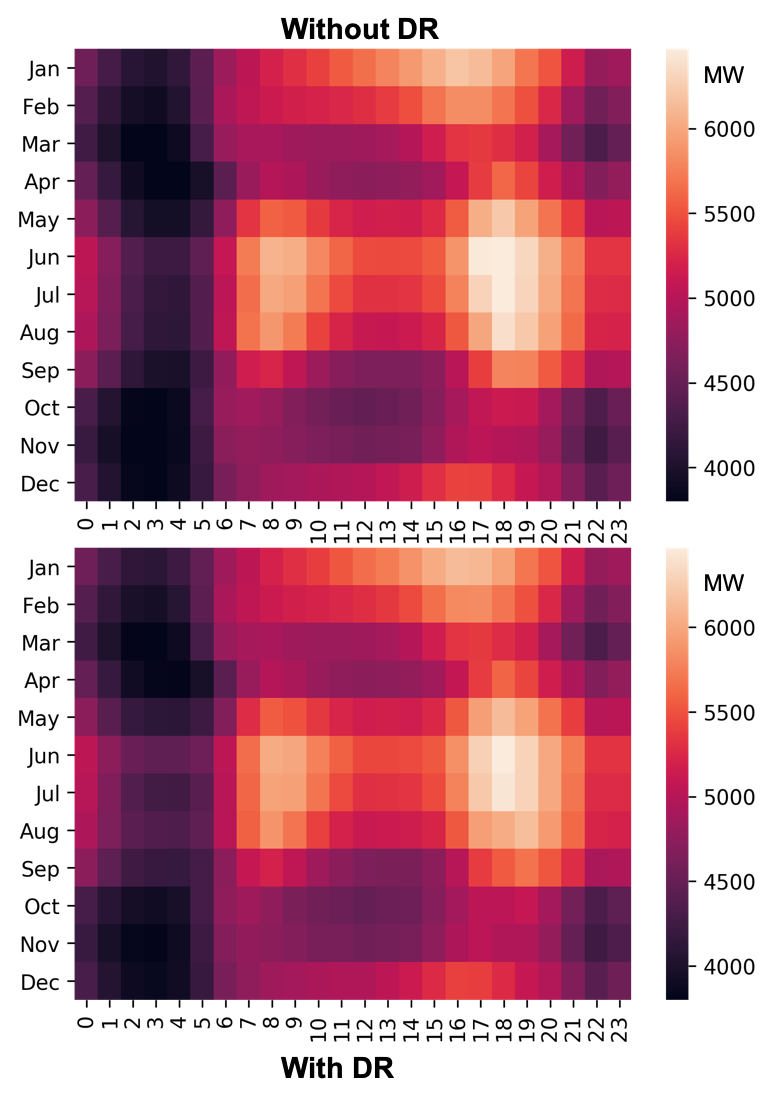
\includegraphics[width=.85\textwidth,height=.51\textheight,keepaspectratio]{DR/PASA_example/Figures_DR/heatmap2018.png}
\caption{Load shifts by hour of day in High DR scenario in 2018}\label{fig:Fig-heatmap}
\end{center}
\end{figure}


\subsection{Results}
\label{sec:dis5.2}

The monthly weighted average demand in Victoria in 2018 is shown in Figure~\ref{fig:Fig-heatmap}. This chart visualises the essence of demand shifted away by time-of-day. This chart displays the time-of-day and the months which electricity is highly consumed. The higher demand periods are mainly clustered in the evening in winter months, summer peaks apparently have less magnitude compared to winter peaks.
From Figure~\ref{fig:Fig-heatmap}, the difference between the pristine dataset without DR and the modelled data can thus be justified by the white cluster which is darken (in modelled DR data) as a result of the load shifting model.

\begin{figure*}
\begin{center}
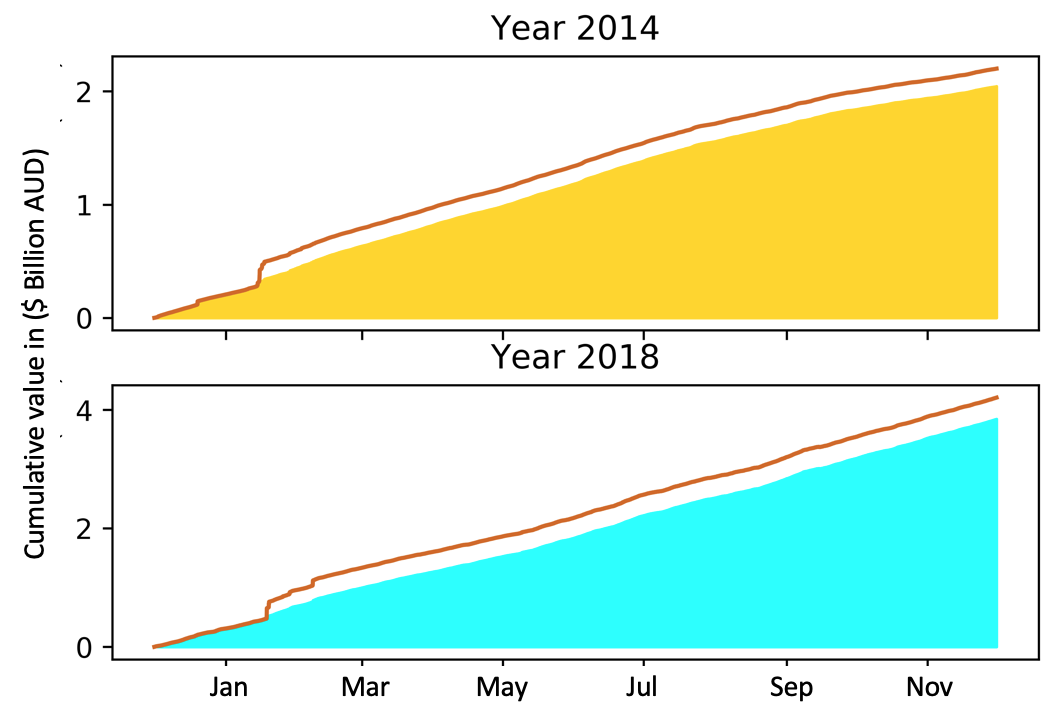
\includegraphics[width=.9\textwidth,height=.5\textheight,keepaspectratio]{DR/PASA_example/Figures_DR/result01.png}
\caption{Model performance based on reduced cumulative market expenditures in 2014 and 2018}\label{fig:Figmodelperformance}
\end{center}
\end{figure*}

Despite the fact that the NEM is the energy-only market which is similar to other electricity market regions e.g. ERCOT in the US or EMA Singapore \cite{ercot2017,ema2014}, load duration curve in Victoria (see Figure~\ref{fig:Fig3-loadcurve}) shows a substantial sharp jump at the very top tier that led to the higher overall prices. Although the price jump occurs only 390 hours or just 4.4\% of the annual operating hours, it attributes to the exponential increase in market value around 14\% of the total market expenditure.

Figure~\ref{fig:Figmodelperformance} shows the historical cumulative volume weighted average price plotted against the modelled cumulative value achieved by this model. Based on this approach, the model delivered similar outputs which can be seen that savings are predominantly obtained by extreme events. A more careful analysis revealed that the annual market expenditure between the two respective years has nearly doubled within 4 years. The rise in electricity prices were largely owing to tighter baseload supply, and increase of gas prices which are conceivably to be the peak prices and the price setters of the market.

Even though the model yielded a reasonably similar pattern, the slope of 2018 (shown in the bottom chart) shows a slight divergence during July to September due to winter's DR potential. As can be seen in Figure~\ref{fig:Figmodelperformance}, the modelled total expenditure in 2014 was \$2.04 billion AUD, compared to historical traded expenditure of \$2.2 billion AUD (7\% potential savings from the model). Higher potential savings gained in 2018 with the modelled traded expenditure of \$3.61 billion AUD, compared to the actual traded value of \$4.20 billion AUD (8.6\% potential savings from the model). The price spikes in both years were associated with extreme weather events. In both cases, the use of DR avoided the price spikes. 


\subsection{Impact analysis on load and price changes}
\label{sec:dis5.3}

This section analyses how results change when the DR potentials are varied as inputs of the model.

\begin{unnumlist}
  \item Baselines:
    The total electricity demand of the Victorian electricity customers and prices associated at half-hourly spot prices in 2014 and 2018. From Table~\ref{table2}, it is noteworthy that the spot market characteristic between the two years has a subtle different especially during high demand periods. Tighter supply side has pushed the generation fleet to bid at higher prices.
  \item Low DR scenario:
    In this scenario analysis, we integrated DR into the market only slightly. When adding an inconsiderable amount of DR (around 3\% of the 10 PoE), the 2014 dataset yielded a comparable potential saving with the 2018's dataset. Potential market expenditures of around 5.4 - 5.8\% can be reduced under this scenario in 2014 and 2018, respectively.
  \item Moderate DR scenario:
    This scenario is set by default and used to analyse the general results and outcomes of the model. This scenario is assumed based on an attainable 5-6\% of DR participation in Victoria. In this simulation, the evaluation based on historical data in 2014 and 2018 brought in the potential cost volatility reduction by 7.1\% and 8.6\%.
  \item High DR scenario:
    In addition to the usual operation of DR, this scenario is granted that DR is readily available in the NEM and there are demand response providers who actively participate in the spot market. This study assumes the maximum DR potential of 950 MW representing an equivalent 10\% of 1-in-10-year probability of exceedance forecast between 2020-22. \footnote{Probability of Exceedance (POE) is a generalised approach to defining the probability of exceedance of electricity demand forecasts E.g. 10\% POE demand implies there is a 10\% probability of the forecast being met or exceeded.} \cite{aemoesoo2017}. This figure is in good agreement with a recent preliminary study in Germany which found that around 10\% of load proportional to the peak demand can be used as DR. Given the maximum penetration of DR potential, the modelled market responded in the expenditures reduction of 8\% and 10.5\% in 2014 and 2018, respectively.
\end{unnumlist}


\begin{figure*}
\begin{center}
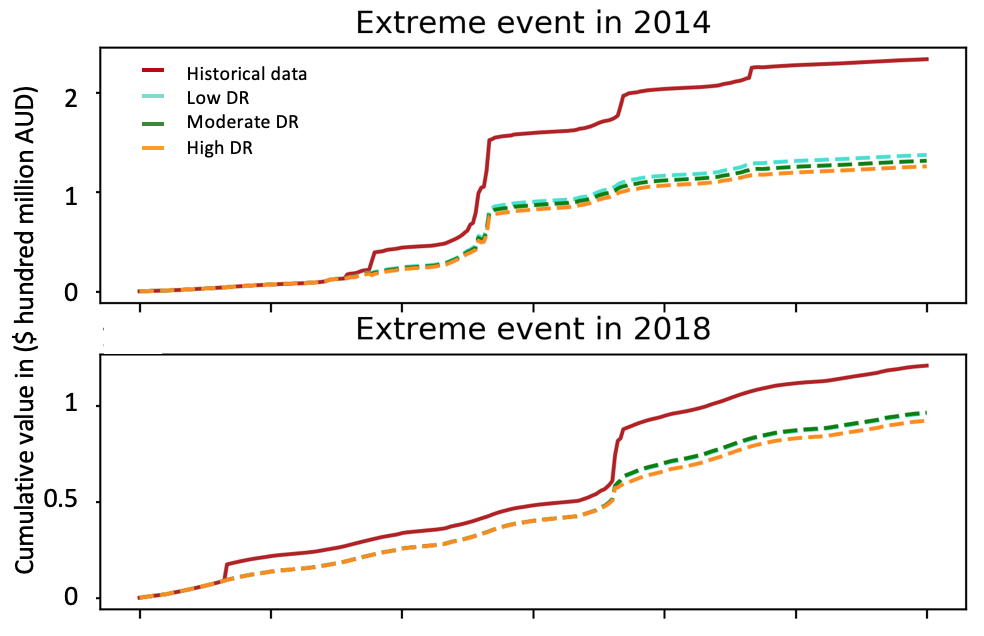
\includegraphics[width=.9\textwidth,height=.6\textheight,keepaspectratio]{DR/PASA_example/Figures_DR/extreme_30.png}
\caption{The potential savings from demand response in extreme weather events modelled against historical data in 2014 and 2018}\label{fig:Figpotentialsavings}
\end{center}
\end{figure*}

Simulations were carried out from 300 to 950 MW availability of DR in 350 MW increments. Based on our scenario analysis, each scenario is granted based on the amount of shiftable power threshold. To demonstrate the performance of the model, data from extreme weather events in 2014 and 2018 are utilised. Figure~\ref{fig:Figpotentialsavings} presents simulations of load shifting impacts ranging from 300 to 950 MW versus two heat wave events in 2014 and 2018. From Figure~\ref{fig:Figpotentialsavings}, model outcomes reveal the level of price surges during the event period. As detailed can be seen in Figure~\ref{fig:Figpotentialsavings}, prices are "jumped" during heat wave periods of six days in 2014 and 2018. When putting DR into perspective, the model yielded potential savings with the spot market value of \$27M  (16\% of the annual saving) during short heat wave event in 2018. While, this figure is dwarfed by the bigger weather event in 2014 which led to substantial cost savings of \$101M or around (75\% of the potential annual saving). 

\begin{figure*}
\begin{center}
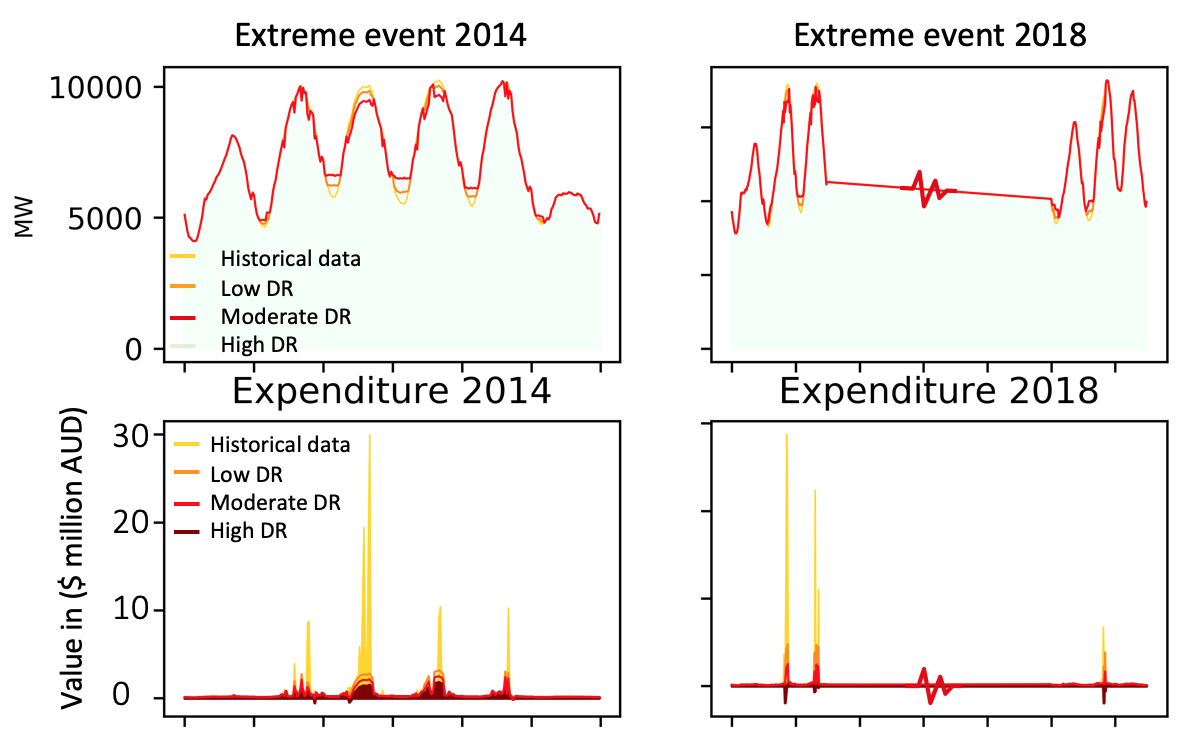
\includegraphics[width=.9\textwidth,height=.6\textheight,keepaspectratio]{DR/PASA_example/Figures_DR/extreme_4grids.png}
\caption{Demand and expenditure impacts from DR modelling in  2014 and 2018}\label{fig:Figdemandexpense}
\end{center}
\end{figure*}

Figure~\ref{fig:Figdemandexpense} illustrates the shifted demand and prices from the effect of modelled DR under extreme weather events. The shaded area of the top charts represents High DR scenario, which can be noticeable that demand is shifted from the peaks to the points in time where the demand is lower. Since electricity demand is inelastic especially during high demand periods, a fraction of shifted demand during this period results in a substantial drop of prices. (as displayed in the bottom charts).

\begin{table*}
\caption{Summary of sensitivity analysis comparing proportional reductions in the total market expenditures and peak costs benefits from Demand Response (DR) usage in 2014 and 2018 across different scenarios.} 
\begin{center}
\begin{tabular*}{\textwidth}{@{}l\x l\x l\x l\x l\x l\x l@{}}
\hline 
\multicolumn{1}{c}{} & \multicolumn{3}{c}{2014}       & \multicolumn{3}{c}{2018} \\ \cline{2-7}
\multicolumn{1}{c}{SCENARIO} & Expenditures & \multicolumn{1}{c}{Potential savings} & \multicolumn{1}{c}{(\%)} & \multicolumn{1}{c}{Expenditures} & \multicolumn{1}{c}{Potential savings} & \multicolumn{1}{c}{(\%)} \\ \cline{2-7}
\multicolumn{1}{c}{} & \multicolumn{1}{c}{(\$)} & \multicolumn{1}{c}{(\$)} & \multicolumn{1}{c}{Change} & \multicolumn{1}{c}{(\$)} & \multicolumn{1}{c}{(\$)} & \multicolumn{1}{c}{Change} \\
 
\hline
Baselines & 2.20$\times10^9$  & ~      & ~   & 4.20$\times10^9$  & ~   & ~ \\ 
Low DR (300MW)   & 2.08$\times10^9$  & 1.2$\times10^8$ & 5.4 & 3.96$\times10^9$ & 2.44$\times10^8$ & 5.8 \\ 
Moderate DR (600MW)& 2.04$\times10^9$ & 1.6$\times10^8$ & 7.1 & 3.84$\times10^9$ & 3.61$\times10^8$ & 8.6 \\
High DR (950MW)  & 2.02$\times10^9$  & 1.8$\times10^8$ & 8.0 & 3.77$\times10^9$ & 4.39$\times10^8$ & 10.5 \\
\hline 
\end{tabular*}\label{table2}
\end{center}
\tabnote{$^a$This is an example of table footnote}
\end{table*}

The overall potential market expenditures will decrease with
increasing level of DR participation (Table~\ref{table2}). Considering the maximum DR potential of 950 MW implemented in 2014, the market could have saved almost \$180 million AUD from the spot market. In 2018, a significantly higher magnitude of saving can be achieved with the accumulate value of \$439 million AUD, representing 10.5\% of the total traded expenditure in that year. 

The most intriguing findings are subsequently presented in Figure~\ref{fig:Figrollingmean}. Since our model allows demand to be shifted within 24 hours (forward or backward within 24-hour time window, described in Section~\ref{loadbalancing}), the two-day moving average plot would best capture the weighted average prices pattern. As can be seen in Figure~\ref{fig:Figmovingavg}, the market responded differently to the identical levels of DR integration. While the effects of different DR integration in 2014 seem to be in a cluster, the effects of different DR scenarios in 2018 otherwise reveal a discrete set of results which could have a meaningful impact on the policy implications.

The potential saving disparities between the two respective years can be found due to the different price characteristics in the spot market. As highlighted in the top chart of Figure~\ref{fig:Figrollingmean}, the marginal difference in expenditure savings of each additional capacity of DR reflects the paradoxical nature of the spot market when supply is abundant --- this contradicts the aforementioned mean-reverting theory that prices should have been exponentially increased in case of higher demand. Nonetheless, there is a number of occurrences which demand and price are not complementing each other in 2014. In other word, although demand are higher than our constraint threshold (8,500 MW), the prices are bid as low as 50 \$/MWh which is below weighted average wholesale price. This circumstance leads to smaller disparities between scenarios as fewer bids were superseded by cheaper DR alternative.


\begin{figure*}
\begin{center}
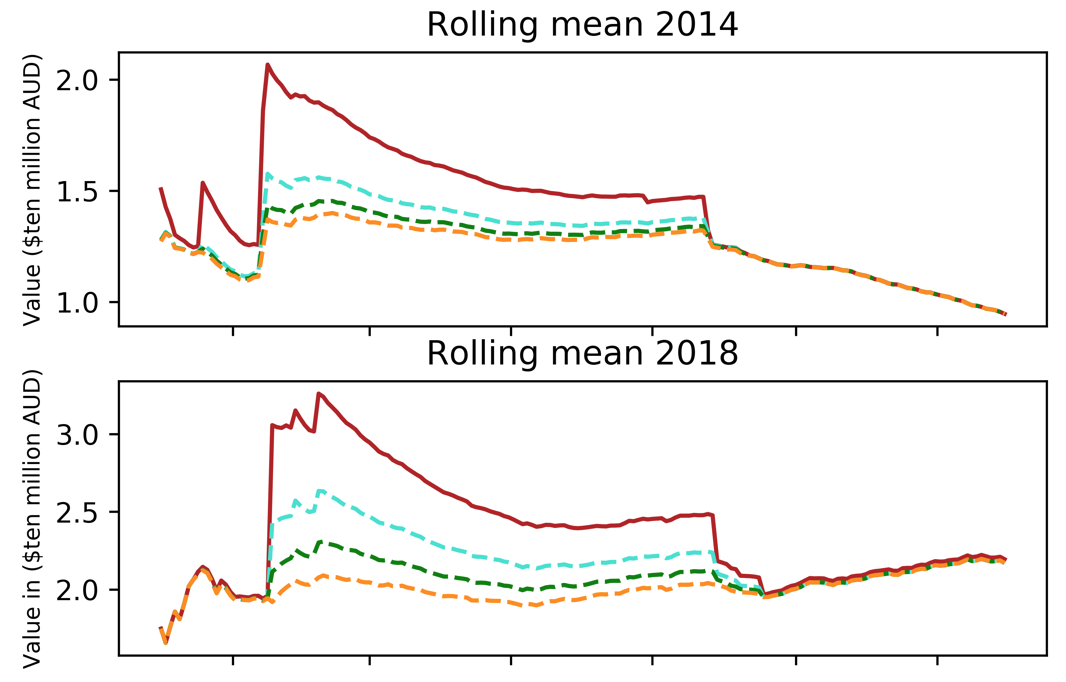
\includegraphics[width=.9\textwidth,height=.6\textheight,keepaspectratio]{DR/PASA_example/Figures_DR/rollingmean.png}
\caption{Two days moving average of market expenditures in 2014 and 2018}\label{fig:Figrollingmean}
\end{center}
\end{figure*}



\section{Conclusion and Policy implications}

This section presents a brief summary extracted from our model outlook, and followed by some interpretation of pragmatic findings that could be the keys for future developments of DR in the Australian National Electricity Market.

Due to retiring baseload power generation and rising costs of fuel for peak power generation, integration of demand response in the energy system has substantial economic value for the Australian National Electricity Market. It also helps the market operator mitigating issues of reliability when supply is tight. This study aims at demonstrating the impact of DR on the merit based spot electricity market under two unique market conditions -- plenty of supply (before the decommission of 1,600~MW coal-fired power plant in 2014) and tighter supply (in 2018).  

As demonstrated in our analysis, the model shows that the integration of flexible demand of 600 MW to the generation fleet in Victoria could have been translating to 7.1\% and 8.6\% reduction of the total value traded the wholesale market in 2014 and 2018, respectively. While increasing the penetration of flexible load to the maximum (950 MW) gives the system better security of supply, the potential reduction in overall system costs is shrunk in comparison to lower penetration of DR. This can be further elaborated as when DR capacity increases, peak demand periods reduce in magnitude and frequency, and DR essentially begins substituting cheaper baseload options rather than higher cost peak generation.

In tighter supply situation, the impacts of load shifting is more pronounced as the peak load plants are triggered more often. In this stance, our simulations deployed economical DR substantially more often than the market with sufficient supply.

Currently, Demand-side Response is broadly considered as reliability and emergency reserve in the NEM. Given that the current DR programs are largely used voluntarily motivational approaches and channelled them through electricity retailers, the cost of DR per MW recruited is not economically viable \cite{oakley2019}. Following on a recent rule change \footnote{This rule change seeks to facilitate wholesale DR, in which customers / aggregators are able to provide direct load to a third party who is able to bid demand reductions into the wholesale market as a substitute for electricity generation.} and proposed amendment of spot market price frequency \footnote{On 1 July 2021, the settlement period for the electricity spot price will change from 30 minutes to five minutes to align operational dispatch and financial settlement.}, DR is likely to deliver a cost effective option in the wholesale spot market. In fact, our evaluation reveals that a level of utilisable of around 300 to 600 MW is preferable especially when demand surges or tighter planned supply.

These results indicate a high potential for electricity end-use customers to exploit this type of behind the meter generation potential that is in line with the contemporaneous rules enacted by Victorian government. 

However, this paper does not reflect the true costs of demand response measures i.e. shifting demand, pricing based demand response or direct load control. In conjunction with the costs, the shifting duration is omitted and assumed to be instantaneous.


\iffalse
\paragraph{This is an example of head level 4.}
Now we are engaged in a great civil war, testing whether that nation, or any nation, so conceived, and so dedicated, can long endure. We are met here on a great battlefield of that war. We have come to dedicate a portion of it as a final resting place for those who here gave their lives that that nation might live. It is altogether fitting and proper that we should do this.
%%%
\begin{verse}
 There is an environment 
 for verse \\ 
 Whose features some poets % within a stanza.
 will curse. 

 For instead of making\\
 Them do \emph{all} line breaking, \\
 It allows them to put too many words on a line when they'd rather be 
 forced to be terse.
\end{verse} 


\begin{itemize}
\item This is a longer itemize list. It consists of two paragraphs of text, neither of which are particularly interesting {\sc ii}.
\item This is a longer itemize list. It consists of two paragraphs of text, neither of which are particularly interesting.
\item This is a longer itemize list. It consists of two paragraphs of text, neither of which are particularly interesting.
\end{itemize}

Now we are engaged in a great civil war, testing whether that nation, or any nation, so conceived, and so dedicated, can long endure. We are met here on a great battlefield of that war. We have come to dedicate a portion of it as a final resting place for those who here gave their lives that that nation might live. It is altogether fitting and proper that we should do this.

\begin{enumerate}%
\item This is a longer numbered list. It consists of two paragraphs of text, neither of which are particularly interesting.
\item This is a short numbered list. It consists of two paragraphs of text.
\end{enumerate}


\begin{figure*}
\begin{center}

\includegraphics[width=30pc, height=12pc]{fpo.eps}
\caption{It is rather for us to be here dedicated to the great task remaining before us  that from these honoured dead we take increased devotion to that cause for which $x^{(0)}=x_1$ and $x^{(0)}=x_2$, where $x_1=(\frac{1}{\sqrt{3,522}},\dots,\frac{1}{\sqrt{3,522}})^T$ and $x_2=(\frac{1}{\sqrt{1,000}}, \dots, \frac{1}{\sqrt{1,000}},0,\dots,0)^T $. they here gave the last full measure of devotion  that we here highly resolve that these dead shall not have died in vain; that this nation shall have a new birth of freedom; and that this government of the people, by the people, for the people, shall not perish from the earth $(x^{(0)})^Tx^{(0)}=1$.}
 \label{Fig11}
\end{center}
\end{figure*}

It is for us, the living, rather to be dedicated here to the \fi



\begin{acknowledgements}
This is a multiline text of acknowledgments. We are met here on a great battlefield of that war. We have come to dedicate a portion of it as a final resting place for those who here gave their lives that that nation might live.
\end{acknowledgements}

\iffalse
\begin{appendix}

\section{AN EXAMPLE OF APPENDIX HEAD}

 Consider a data set
\begin{equation}
S=(f_{ij})_{m\times n}
\end{equation} the \(i\)th
data point of which is
\[ (f_{i1}, . . . , f_{in}).\]
 Let $\overline{f}_q=\frac{1}{m}\sum_{i=1}^mf_{iq}$ and $\sigma_q$ The brave men, living and dead, who struggled, here, have consecrated it far above our poor power to add or detract. Suppose that
\[X_i=(x_{i1},\dots,x_{in}) \indent (i=1,\dots, m),\]  
where $x_{ij}=(f_{ij}-\overline{f}_j)/\sigma_j $ and
\[B=(X_1^T,\dots,X_m^T)^T.\]
 Then we can show that
\[C=B^TB=\sum\limits_{i=1}^m X_i^TX_i=(C_{jk})_{n\times n},\]
where $C_{jk}=\sum_{i=1}^mx_{ij}x_{ik}$ is the correlation matrix. Our goal is to find a normalized vector 
$$a_1=(a_{11},a_{12},\dots,a_{1n})^T$$
 such that the projection of the standardized data
\[X_ia_1=\sum\limits_{k=1}^n x_{ik}a_{1k},\]
\noindent then $Ba_1$ 
 \[a_1^TB^T �� Ba_1=a_1^TCa_1.\]
 Our goal is to maximize this value under the constraint $a_1^Ta_1=1$. Let $\lambda_{\rm max}$ be the largest eigenvalue of
 $C$. According to the Rayleigh--Ritz theorem, $a_1$ can be obtained by solving
 \[Ca_1= \lambda_{\rm max}a_1.\]
But in a larger sense we can not dedicate -- we can not consecrate -- we can not hallow this ground. The brave men, living and dead, who struggled, here, have consecrated it far above our poor power to add or detract. The world will little note, nor long remember, what we say here, but can never forget what they did here. It is for us, the living, rather to be dedicated here to the unfinished work which they have, thus far, so nobly carried on \cite{abt1981}. It is rather for us to be here dedicated to the great task remaining before us  that from these honoured dead we take increased devotion to that cause for which they here gave the last full measure of devotion  that we here highly resolve that these dead shall not have died in vain; that this nation shall have a new birth of freedom; and that this government \cite{abt1984b} of the people, by the people, for the people, shall not perish from the earth.
\end{appendix}

\fi
% UNCOMMENT THE LINES BELOW IF YOU WISH TO USE BIBTEX
%\bibliographystyle{apj}
%\bibliography{yourbibfile}

%%\begin{thebibliography}{}
%%
%%\bibitem[\protect\citename{Afanas'ev et al. }1990]{afa}
%%Afanas'ev, V. L., Vlasyuk, V. V., Dodonov, S. N., Lorentz, H., \& Terebizh, V. 1990, BSAO, 32, 51
%%
%%\bibitem[\protect\citename{Arp \& Duhalde }1985]{arp}
%%Arp, H., \& Duhalde, O. 1985, PASP, 97, 1149
%%
%%\bibitem[\protect\citename{Burbidge, Crowne, \& Smith }1977]{bcs}
%%Burbidge, G. R., Crowne, A. H., \& Smith, H. E. 1977, ApJS, 33, 113
%%
%%\bibitem[\protect\citename{Campusano \& Pedreros }1978]{cp}
%%Campusano, L. E., \& Pedreros, M. 1978, Obs. Astron. Natl. Cerro Calan (Santiago: Dep. Astron. Publ. III), 315
%%
%%\bibitem[\protect\citename{Flesch }2010]{fls}
%%Flesch, E. 2010, PASA, 27, 283
%%
%%\bibitem[\protect\citename{Knuth }1984]{DEK84}
%%Knuth,~D.~E. 1984, Obs. Astron. Natl. Cerro Calan (Santiago: Dep. Astron. Publ. III), 315
%%
%%\bibitem[\protect\citename{Lamport }1986]{LaTeX}
%%Lamport,~L. 1986, \LaTeX: A Document Preparation System (2nd edn; New York: Addison-Wesley) 
%%
%%\bibitem[\protect\citename{Lanzetta et al. }1991]{lwt}
%%Lanzetta, K. M., Wolfe, A. M., Turnshek, D. A., Lu, L., McMahon, R. G., \& Hazard, C. 1991, ApJS, 77, 1
%%
%%\bibitem[\protect\citename{Reichert et al. }1982]{rmt}
%%Reichert, G. A., Mason, K. O., Thorstensen, J. R., \& Bowyer, S. 1982, ApJ, 260, 437
%%
%%\bibitem[\protect\citename{Remillard }1993]{rem}
%%Remillard, R. A., et al. 1993, AJ, 105, 2079
%%
%%\bibitem[\protect\citename{Sargent, Boksenberg, \& Steidel }1993]{sbs}
%%Sargent, W. L., Boksenberg, A., \& Steidel, C. C. 1988, ApJS, 68, 539
%%
%%\bibitem[\protect\citename{Wolfe et al. }1986]{wts}
%%Wolfe, A. M., Turnshek, D. A., Smith, H. E., \& Cohen, R. D. 1986, ApJS, 61, 249
%%
%%\end{thebibliography}

\nocite*{}
\bibliography{DR_cite}

\end{document}
